
%% bare_conf.tex
%% V1.4b
%% 2020/01/30
%% by WenbinLi
%% See:
%% http://www.michaelshell.org/
%% for current contact information.
%%
%% This is a skeleton file demonstrating the use of IEEEtran.cls
%% (requires IEEEtran.cls version 1.8b or later) with an IEEE
%% conference paper.
%%
%% Support sites:
%% http://www.michaelshell.org/tex/ieeetran/
%% http://www.ctan.org/pkg/ieeetran
%% and
%% http://www.ieee.org/

%%*************************************************************************
%% Legal Notice:
%% This code is offered as-is without any warranty either expressed or
%% implied; without even the implied warranty of MERCHANTABILITY or
%% FITNESS FOR A PARTICULAR PURPOSE! 
%% User assumes all risk.
%% In no event shall the IEEE or any contributor to this code be liable for
%% any damages or losses, including, but not limited to, incidental,
%% consequential, or any other damages, resulting from the use or misuse
%% of any information contained here.
%%
%% All comments are the opinions of their respective authors and are not
%% necessarily endorsed by the IEEE.
%%
%% This work is distributed under the LaTeX Project Public License (LPPL)
%% ( http://www.latex-project.org/ ) version 1.3, and may be freely used,
%% distributed and modified. A copy of the LPPL, version 1.3, is included
%% in the base LaTeX documentation of all distributions of LaTeX released
%% 2003/12/01 or later.
%% Retain all contribution notices and credits.
%% ** Modified files should be clearly indicated as such, including  **
%% ** renaming them and changing author support contact information. **
%%*************************************************************************


% *** Authors should verify (and, if needed, correct) their LaTeX system  ***
% *** with the testflow diagnostic prior to trusting their LaTeX platform ***
% *** with production work. The IEEE's font choices and paper sizes can   ***
% *** trigger bugs that do not appear when using other class files.       ***                          ***
% The testflow support page is at:
% http://www.michaelshell.org/tex/testflow/



\documentclass[conference]{IEEEtran}
% Some Computer Society conferences also require the compsoc mode option,
% but others use the standard conference format.
%
% If IEEEtran.cls has not been installed into the LaTeX system files,
% manually specify the path to it like:
% \documentclass[conference]{../sty/IEEEtran}





% Some very useful LaTeX packages include:
% (uncomment the ones you want to load)


% *** MISC UTILITY PACKAGES ***
%
%\usepackage{ifpdf}
% Heiko Oberdiek's ifpdf.sty is very useful if you need conditional
% compilation based on whether the output is pdf or dvi.
% usage:
% \ifpdf
%   % pdf code
% \else
%   % dvi code
% \fi
% The latest version of ifpdf.sty can be obtained from:
% http://www.ctan.org/pkg/ifpdf
% Also, note that IEEEtran.cls V1.7 and later provides a builtin
% \ifCLASSINFOpdf conditional that works the same way.
% When switching from latex to pdflatex and vice-versa, the compiler may
% have to be run twice to clear warning/error messages.






% *** CITATION PACKAGES ***
%
%\usepackage{cite}
% cite.sty was written by Donald Arseneau
% V1.6 and later of IEEEtran pre-defines the format of the cite.sty package
% \cite{} output to follow that of the IEEE. Loading the cite package will
% result in citation numbers being automatically sorted and properly
% "compressed/ranged". e.g., [1], [9], [2], [7], [5], [6] without using
% cite.sty will become [1], [2], [5]--[7], [9] using cite.sty. cite.sty's
% \cite will automatically add leading space, if needed. Use cite.sty's
% noadjust option (cite.sty V3.8 and later) if you want to turn this off
% such as if a citation ever needs to be enclosed in parenthesis.
% cite.sty is already installed on most LaTeX systems. Be sure and use
% version 5.0 (2009-03-20) and later if using hyperref.sty.
% The latest version can be obtained at:
% http://www.ctan.org/pkg/cite
% The documentation is contained in the cite.sty file itself.






% *** GRAPHICS RELATED PACKAGES ***
%
\ifCLASSINFOpdf
  % \usepackage[pdftex]{graphicx}
  % declare the path(s) where your graphic files are
  % \graphicspath{{../pdf/}{../jpeg/}}
  % and their extensions so you won't have to specify these with
  % every instance of \includegraphics
  % \DeclareGraphicsExtensions{.pdf,.jpeg,.png}
\else
  % or other class option (dvipsone, dvipdf, if not using dvips). graphicx
  % will default to the driver specified in the system graphics.cfg if no
  % driver is specified.
  % \usepackage[dvips]{graphicx}
  % declare the path(s) where your graphic files are
  % \graphicspath{{../eps/}}
  % and their extensions so you won't have to specify these with
  % every instance of \includegraphics
  % \DeclareGraphicsExtensions{.eps}
\fi
% graphicx was written by David Carlisle and Sebastian Rahtz. It is
% required if you want graphics, photos, etc. graphicx.sty is already
% installed on most LaTeX systems. The latest version and documentation
% can be obtained at: 
% http://www.ctan.org/pkg/graphicx
% Another good source of documentation is "Using Imported Graphics in
% LaTeX2e" by Keith Reckdahl which can be found at:
% http://www.ctan.org/pkg/epslatex
%
% latex, and pdflatex in dvi mode, support graphics in encapsulated
% postscript (.eps) format. pdflatex in pdf mode supports graphics
% in .pdf, .jpeg, .png and .mps (metapost) formats. Users should ensure
% that all non-photo figures use a vector format (.eps, .pdf, .mps) and
% not a bitmapped formats (.jpeg, .png). The IEEE frowns on bitmapped formats
% which can result in "jaggedy"/blurry rendering of lines and letters as
% well as large increases in file sizes.
%
% You can find documentation about the pdfTeX application at:
% http://www.tug.org/applications/pdftex





% *** MATH PACKAGES ***
%
%\usepackage{amsmath}
% A popular package from the American Mathematical Society that provides
% many useful and powerful commands for dealing with mathematics.
%
% Note that the amsmath package sets \interdisplaylinepenalty to 10000
% thus preventing page breaks from occurring within multiline equations. Use:
%\interdisplaylinepenalty=2500
% after loading amsmath to restore such page breaks as IEEEtran.cls normally
% does. amsmath.sty is already installed on most LaTeX systems. The latest
% version and documentation can be obtained at:
% http://www.ctan.org/pkg/amsmath





% *** SPECIALIZED LIST PACKAGES ***
%
%\usepackage{algorithmic}
% algorithmic.sty was written by Peter Williams and Rogerio Brito.
% This package provides an algorithmic environment fo describing algorithms.
% You can use the algorithmic environment in-text or within a figure
% environment to provide for a floating algorithm. Do NOT use the algorithm
% floating environment provided by algorithm.sty (by the same authors) or
% algorithm2e.sty (by Christophe Fiorio) as the IEEE does not use dedicated
% algorithm float types and packages that provide these will not provide
% correct IEEE style captions. The latest version and documentation of
% algorithmic.sty can be obtained at:
% http://www.ctan.org/pkg/algorithms
% Also of interest may be the (relatively newer and more customizable)
% algorithmicx.sty package by Szasz Janos:
% http://www.ctan.org/pkg/algorithmicx




% *** ALIGNMENT PACKAGES ***
%
%\usepackage{array}
% Frank Mittelbach's and David Carlisle's array.sty patches and improves
% the standard LaTeX2e array and tabular environments to provide better
% appearance and additional user controls. As the default LaTeX2e table
% generation code is lacking to the point of almost being broken with
% respect to the quality of the end results, all users are strongly
% advised to use an enhanced (at the very least that provided by array.sty)
% set of table tools. array.sty is already installed on most systems. The
% latest version and documentation can be obtained at:
% http://www.ctan.org/pkg/array


% IEEEtran contains the IEEEeqnarray family of commands that can be used to
% generate multiline equations as well as matrices, tables, etc., of high
% quality.




% *** SUBFIGURE PACKAGES ***
%\ifCLASSOPTIONcompsoc
%  \usepackage[caption=false,font=normalsize,labelfont=sf,textfont=sf]{subfig}
%\else
%  \usepackage[caption=false,font=footnotesize]{subfig}
%\fi
% subfig.sty, written by Steven Douglas Cochran, is the modern replacement
% for subfigure.sty, the latter of which is no longer maintained and is
% incompatible with some LaTeX packages including fixltx2e. However,
% subfig.sty requires and automatically loads Axel Sommerfeldt's caption.sty
% which will override IEEEtran.cls' handling of captions and this will result
% in non-IEEE style figure/table captions. To prevent this problem, be sure
% and invoke subfig.sty's "caption=false" package option (available since
% subfig.sty version 1.3, 2005/06/28) as this is will preserve IEEEtran.cls
% handling of captions.
% Note that the Computer Society format requires a larger sans serif font
% than the serif footnote size font used in traditional IEEE formatting
% and thus the need to invoke different subfig.sty package options depending
% on whether compsoc mode has been enabled.
%
% The latest version and documentation of subfig.sty can be obtained at:
% http://www.ctan.org/pkg/subfig




% *** FLOAT PACKAGES ***
%
%\usepackage{fixltx2e}
% fixltx2e, the successor to the earlier fix2col.sty, was written by
% Frank Mittelbach and David Carlisle. This package corrects a few problems
% in the LaTeX2e kernel, the most notable of which is that in current
% LaTeX2e releases, the ordering of single and double column floats is not
% guaranteed to be preserved. Thus, an unpatched LaTeX2e can allow a
% single column figure to be placed prior to an earlier double column
% figure.
% Be aware that LaTeX2e kernels dated 2015 and later have fixltx2e.sty's
% corrections already built into the system in which case a warning will
% be issued if an attempt is made to load fixltx2e.sty as it is no longer
% needed.
% The latest version and documentation can be found at:
% http://www.ctan.org/pkg/fixltx2e


%\usepackage{stfloats}
% stfloats.sty was written by Sigitas Tolusis. This package gives LaTeX2e
% the ability to do double column floats at the bottom of the page as well
% as the top. (e.g., "\begin{figure*}[!b]" is not normally possible in
% LaTeX2e). It also provides a command:
%\fnbelowfloat
% to enable the placement of footnotes below bottom floats (the standard
% LaTeX2e kernel puts them above bottom floats). This is an invasive package
% which rewrites many portions of the LaTeX2e float routines. It may not work
% with other packages that modify the LaTeX2e float routines. The latest
% version and documentation can be obtained at:
% http://www.ctan.org/pkg/stfloats
% Do not use the stfloats baselinefloat ability as the IEEE does not allow
% \baselineskip to stretch. Authors submitting work to the IEEE should note
% that the IEEE rarely uses double column equations and that authors should try
% to avoid such use. Do not be tempted to use the cuted.sty or midfloat.sty
% packages (also by Sigitas Tolusis) as the IEEE does not format its papers in
% such ways.
% Do not attempt to use stfloats with fixltx2e as they are incompatible.
% Instead, use Morten Hogholm'a dblfloatfix which combines the features
% of both fixltx2e and stfloats:
%
% \usepackage{dblfloatfix}
% The latest version can be found at:
% http://www.ctan.org/pkg/dblfloatfix




% *** PDF, URL AND HYPERLINK PACKAGES ***
%
%\usepackage{url}
% url.sty was written by Donald Arseneau. It provides better support for
% handling and breaking URLs. url.sty is already installed on most LaTeX
% systems. The latest version and documentation can be obtained at:
% http://www.ctan.org/pkg/url
% Basically, \url{my_url_here}.




% *** Do not adjust lengths that control margins, column widths, etc. ***
% *** Do not use packages that alter fonts (such as pslatex).         ***
% There should be no need to do such things with IEEEtran.cls V1.6 and later.
% (Unless specifically asked to do so by the journal or conference you plan
% to submit to, of course. )


% correct bad hyphenation here
\hyphenation{op-tical net-works semi-conduc-tor}

% The preceding line is only needed to identify funding in the first footnote. If that is unneeded, please comment it out.
\usepackage{cite}
\usepackage{amsmath,amssymb,amsfonts}
\usepackage{algorithmic}
\usepackage{graphicx}
\usepackage{float} 
\usepackage{subfigure}
\usepackage{textcomp}
\usepackage{xcolor}
\usepackage{ctex}
\usepackage{booktabs}
\usepackage{caption}
\usepackage[colorlinks]{hyperref}

\usepackage{booktabs,ragged2e}
\usepackage[flushleft]{threeparttable}
\renewcommand\TPTtagStyle{\textit}
\usepackage{tabularx,booktabs}
\newcolumntype{C}{>{\centering\arraybackslash}X} % centered version of "X" type
\setlength{\extrarowheight}{1pt}
\usepackage{lipsum}
\begin{document}
%
% paper title
% Titles are generally capitalized except for words such as a, an, and, as,
% at, but, by, for, in, nor, of, on, or, the, to and up, which are usually
% not capitalized unless they are the first or last word of the title.
% Linebreaks \\ can be used within to get better formatting as desired.
% Do not put math or special symbols in the title.
\title{A Review Of Image Segmentation\\图像分割论文综述}


% author names and affiliations

\author{\IEEEauthorblockN{Wenbin Li}
\IEEEauthorblockA{Student Identification Number: 1120173001\\Email: 1120173001@bit.edu.cn\\
Beijing Institute of Technology
}}
%\and
%\IEEEauthorblockN{Homer Simpson}
%\IEEEauthorblockA{Twentieth Century Fox\\
%Springfield, USA\\
%Email: homer@thesimpsons.com}


% use for special paper notices
%\IEEEspecialpapernotice{(Invited Paper)}

% make the title area
\maketitle

% As a general rule, do not put math, special symbols or citations
% in the abstract
\begin{abstract}
本文的目的是对数字图像分割技术进行综述。图像分割是指将一幅数字图像分割成多段的过程,即一组像素,根据颜色、强度或纹理等同质性准则,区域内的像素是相似的,以便定位和识别图像中的对象和边界。近年来,数字图像分割问题一直是计算机视觉的研究热点。计算机视觉涉及的图像处理问题为数字图像分割的研究开拓了广阔的前景,很多亟待解决的数字图像分割问题也富于挑战。随着对数字图像分割研究的不断深入,针对不同的应用领域,人们对图像的内容分析和理解提出了许多不同的分割方法。因此,有组织地回顾图像分割方法是必要的。本文回顾了2010年-2019年A类期刊文献中提出的各种图像分割技术,并对数字图像分割使用的几种重要算法进行综述,讨论每种算法的主要方法,应用以及优缺点。
\end{abstract}

% no keywords




% For peer review papers, you can put extra information on the cover
% page as needed:
% \ifCLASSOPTIONpeerreview
% \begin{center} \bfseries EDICS Category: 3-BBND \end{center}
% \fi
%
% For peerreview papers, this IEEEtran command inserts a page break and
% creates the second title. It will be ignored for other modes.
\IEEEpeerreviewmaketitle



\section{引言}
% no \IEEEPARstart
在许多应用中,数字图像处理(Digital Image Processing, DIP 为其缩写)在不影响图像其他特征的情况下从给定的图像中检索所需信息方面起着至关重要的作用。图像是传递信息的重要媒介,通过对图像的理解,检索到的信息可以用于许多任务;数字图像是由有限个元素或像素组成的,对图像的采集称为成像。DIP是一种多学科的操作,它具有图像表示、分割、压缩和变换等多种处理过程。
图像分割是图像处理中最重要的任务之一,它将图像分割成若干不相交的子集,使得每个子集对应于图像的有意义部分。图像分割也是图像分析的一个重要组成部分,它是从特定的图像中提取清晰、有意义的信息,以满足应用的需要。
图像分割的实际应用范围包括滤除噪声图像、医学应用(定位肿瘤和其他病理学)、卫星图像中的目标定位(道路、森林等)、人脸识别,指纹识别。分割技术的选择和分割水平取决于所考虑问题的特定类型和特征。

%\hfill mds
 
%\hfill August 26, 2015

\section{分割方法综述}
	图像分割已经成为基于图像应用的一个重要阶段。分割是将一幅数字图像分割成多个区域,并提取出一个有意义的区域,即感兴趣区域的过程。不连续性原理背后的思想是提取不同性质的区域,如强度、颜色、纹理或任何其他图像统计信息。相似性原理的基本思想是基于公共属性对像素进行分组。

\subsection{传统分割方法}

\subsubsection{阈值法}
阈值法中的阈值可以根据先验知识手动选择,也可以通过图像信息自动选择。\\
在与边缘信息相关的边缘算法中,算法又可分为基于边缘的算法、基于区域的算法和混合阈值的算法。常见的边缘检测算法有Canny边缘检测算法和Laplacian边缘检测算法。由于算法的操作是基于像素的,因此检测到的边缘由离散像素组成,因此可能是不完整的或不连续的。因此,有必要采用形态学等后处理方法来连接断裂或消除孔洞。阈值法也试图在消除噪声影响的同时找到边缘像素。例如,Canny边缘检测器使用梯度幅度阈值来寻找潜在边缘像素,并通过抑制共享的过程来抑制噪声。\\阈值法对三维图像具有较好的分割精度,但该方法的缺点是处理纹理块状物体图像困难。
\subsubsection{边缘检测法}边缘在许多图像处理应用中起着非常重要的作用。它们提供了物体的轮廓。边缘是一组连接的像素,位于两个灰度值不同的区域之间的边界上。边缘上的这些像素称为边缘点,通常通过计算图像函数的导数来提取边缘。\\
图像处理中的常见边缘有表示快速变化并立即返回原始强度级别的尖峰边缘,表示强度渐变的台阶边缘等。\\
边缘检测算法主要依据检测图像亮度的剧烈变化,算法流程图如图\ref{img}所示
 \begin{figure}[h]
  \centering
  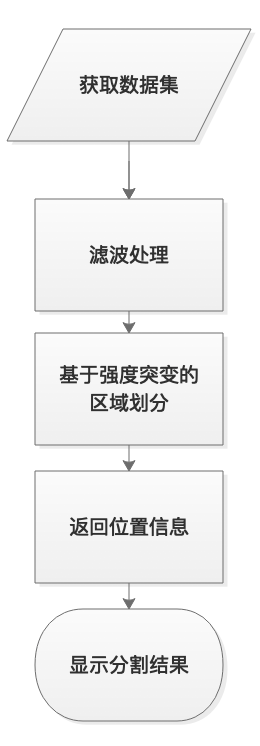
\includegraphics[width=4.0cm,height=10.0cm]{1.png} %1.png是图片文件的相对路径
  \caption{边缘检测流程图} %caption是图片的标题
  \label{img} %此处的label相当于一个图片的专属标志,目的是方便上下文的引用
\end{figure}
\subsubsection{边界生长法}
	与边缘检测方法相比,基于区域的分割算法相对简单,对噪声的免疫能力更强。基于边缘的方法基于边缘附近强度的快速变化对图像进行分割,而基于区域的方法根据一组预定义的标准将图像分割成相似的区域,在基于区域的分割中,与对象相对应的像素被组合在一起并标记。基于区域的分割还需要使用适当的阈值技术。重要的原则是值相似性(包括灰度值差异和灰度值方差)和空间接近度(由区域的欧几里得距离和紧度组成)。本文主要讨论基于区域的边界生长法。
	区域增长提取图像中基于强度信息的图像区域。它通过检测相邻像素并将其加入到一个不检测边缘的区域类中,并对区域中的每个边界像素迭代此过程。如果发现相邻区域,则使用区域合并算法,其中弱边被分解,强边保持完整。
    区域增长方法通过比较图像的灰度、纹理、颜色和形状等各种特性,根据每个像素与其相邻像素的相似性对图像进行分割。该方法的基本思想是将图像中具有相似性质的像素集合进行分组,形成一个区域。在这个方法中,区域通过选择一个叫做种子像素的起点来增长。然后,根据一定的均匀性准则,通过添加相似的邻域像素,逐步增大区域的大小,实现区域的增长。均匀性准则具有决定像素是否属于生长区域的功能。
	区域生长可以分为四个步骤:
\begin{itemize}
\item[1)]标记原始图像中的种子像素组;
\item[2)]选择灰度强度或颜色等聚类准则,并设置停止规则;
\item[3)]通过将每个种子连接到满足类似于种子像素的簇特性的相邻像素来扩展区域;
\item[4)]当不再有像素满足包含在该区域中的标准时,停止区域增长;
\end{itemize}

\subsection{聚类}
聚类算法(Clustering)使用图像的一组相似属性(如像素、颜色和边界)来分割图像。在基于聚类的图像分割中,输入图像根据距离、连通性和强度值等相似性质被分成若干组。在像素之间定义相似性准则,然后将相似像素分组形成簇。将像素分组成簇是基于最大化类内相似性和最大化类间相似性的原理。聚类算法不使用训练数据,而是在分割图像和描述每个类的属性之间迭代。
\subsubsection{类型划分}
聚类技术可分为硬聚类和软聚类两大类。
在硬聚类中,数据被划分为若干个唯一的聚类,其中每个数据组件恰好属于一个聚类。其中最流行和使用最广泛的硬聚类算法是K-means聚类算法[11]。\\在软聚类中,数据元素可以属于多个具有一定关系值的聚类。模糊聚类(Fuzzy C-Means)是一种软聚类算法,可用于图像中不同对象之间没有定义边界的情况。模糊聚类根据距离、连通性、强度等相似性准则将输入像素划分为一个或多个簇.\\
近年来,谱聚类(Spectral Clustering)在生物信息学、信息检索和图像分割等领域得到了成功的应用。谱聚类是一种基于谱图理论的任意形状分割算法;基于光谱的图像分割的目的是将输入图像分割成若干空间相邻、光谱相似的同质区域,并将目标与背景分离[1]。
\subsubsection{K-means}
K-means算法是一种迭代的、数值的、不确定的、无监督的聚类方法,它根据输入数据点之间的固有距离将它们分为多个类。K-means算法是基于数据成分对之间的相似性或相异性指数。
K-means算法假设数据特征形成一个向量空间,并试图在其中找到自然聚类。在这种方法中,像素点围绕聚类中心聚集,聚类中心则通过最小化空间获得的[2]。\\K-means聚类是一种将图像的n个像素聚类成K个簇的技术,(K<n,K为正整数)。聚类中心在算法中是随机初始化的,聚类基于像素灰度强度和像素强度距离等相似性特征形成。
在这种聚类算法中,数据通过计算每个组的强度迭代地进行聚类,并通过用最接近的一个像素对类中的每个像素进行分类来分割图像。使用K-means算法分割图像要遵循的各个步骤如下:
将图像作为输入并计算强度分布。
\begin{itemize}
\item[1)]用k个随机强度初始化质心;

\item[2)]重复步骤,直到目标函数不再改变:
\item[3)]基于其强度与质心强度的距离对点进行聚类,
\item[4)]计算每个簇的新质心;
\end{itemize}
\subsubsection{Fuzzy C-Means}
模糊聚类Fuzzy C-Means(FCM)是一种无监督聚类算法,它通过将特征空间中相似的数据点进行聚类来对图像进行分类。该方法根据输入图像中相似像素的分组,将输入图像分割为区域,并且图像上的像素具有很强的相关性,因此相邻像素的空间关系是图像分割中的一个重要特征。\\
在该聚类算法中,通过对相似像素进行分组,并根据相似特征对组中的每个像素进行分类,从而对数据进行迭代聚类。使用模糊C均值算法分割图像要遵循的各个步骤如下:
\begin{itemize}
\item [a)]其中一个像素作为一组簇的常数放置;
\item [b)]识别像素距离并计算输入图像的给定尺寸;
\item [c)]开始迭代,如果达到可能的迭代,则停止该过程并获得分割图像
\item [d)]否则,继续迭代过程;
\end{itemize}

\subsubsection{Spectral Clustering}
光谱聚类(Spectral Clustering)是一种基于相似度和图论的聚类方法,在图像分割过程中需要计算每对像素之间的相似度。利用谱聚类进行图像分割,可以利用反映数据相似性的相似矩阵特征向量来检测数据的内部结构,并用标准的线性代数方法进行求解。与传统的K-均值聚类方法相比,谱聚类可以对任意形状的样本空间进行聚类。谱聚类分割算法是先建立一个无向图,然后进行多通道分割[3]。\\
基于谱聚类的图像分割提高了图像分割的质量,降低了计算复杂度。谱方法利用数据相似矩阵的特征值来降维,并用于数据点的分组。相似度矩阵作为输入,由与数据集中每对点的相似度相关的定量评估组成。使用光谱聚类算法分割图像要遵循的各个步骤如下:
\begin{itemize}
\item[1)]根据像素级别将图像分割成许多小的同质区域;
\item[2)]对输入图像进行预处理,得到图像特征向量矩阵;
\item[3)]提取图像的颜色、纹理和形状特征,并用提取的特征矩阵计算图像相似度。
\end{itemize}
\subsubsection{算法比较}
如表1所示,为三类聚类算法的比较,并总结各类优缺点;
\begin{table}[h]
\begin{threeparttable}
\label{Tab:1}
\caption{图像分割聚类算法总结与比较}
\centering
\begin{tabular}{lp{3cm}p{3cm}p{3cm}}
\toprule
 \textbf{方法} & \textbf{优点} & \textbf{缺点}\\
%     \multicolumn{4}{c}{Accuracy (\%)} \\ 
%%\cmidrule{3-6}
%     & & K3 & K6 & L1 & mean\tnote{c} \\
\midrule
   K-means & 1)聚类方法简单易快速设计; 2)易于生成特定数量的不相交扁平簇
   & 1)聚类数事先确定; 2)受初始值影响大 \\ \hline
\addlinespace
   Fuzzy C-Means
   & 1)软性隶属后,隶属函数对数据空间进行了适当的划分;
   2)迭代更易达到全局最优;对噪声有一定的鲁棒性
   & 1)相比于K-means,计算复杂度更高; 2)具有和K-means相似的缺点  \\ 
   \hline
\addlinespace
   Spectral Clustering
   & 1)分类效果好; 2)可适当减少计算量;
   & 当图像分辨率较高时,光谱聚类会导致邻接矩阵过大\\
   \hline
  
\bottomrule

\end{tabular}
\end{threeparttable}
\end{table}


\subsection{特殊算法}
基于特殊理论的分割支持不同领域的派生算法,如基于神经网络的算法、基于模糊的算法、基于小波的算法和基于聚类的算法。
\subsubsection{人工神经网络}
神经网络试图模拟人脑的学习过程,是人脑的一种人工表示。人工神经网络通常被称为神经网络。\\近年来,人工神经网络被广泛应用于解决医学图像分割问题。基于生命模拟的神经网络,特别是人脑的学习过程,可以构成大量的并行节点,每个节点都可以执行一些基本计算。而神经网络结构的学习过程可以通过传递节点之间的连接和连接权重来实现。神经网络的主要优点是不依赖于概率密度分布函数,当数据偏离正常情况时,也能证明分割结果。此外,神经网络还可以降低图像分割过程中人为干预因素产生的不良影响。\\
人工神经网络结构通常由模拟神经元的节点和带有权值的连接网络组成,每个节点都可以执行一些基本计算,学习过程可以通过节点间的连接转移和连接权值来实现。在基于神经网络的图像分割中,首先将图像转化为能量最小化,然后利用训练样本集对神经网络进行训练,确定节点之间的连接和权值。\\
近两年,随着科技医疗的发展,神经网络在医学图像分割中得到了广泛的应用,降低了医学图像分割过程中人为因素对图像处理的干扰。\\
在神经网络中,每个神经元对应一幅图像的像素,并将图像映射到神经网络中。利用训练样本对神经网络形式的图像进行训练,找到神经元(即像素)之间的连接。然后从训练后的图像中分割出新的图像。用于图像分割的各种神经网络有Hopfield、BPNN、FFNN、MLFF、MLP、SOM和PCNN。在神经网络中,图像被视为图像数据均匀的段的组合,用于确定图像段的两个因素是[4]:
\begin{itemize}
\item [1] 满足均匀性准则的所有像素的分类;
\item [2] 检测不同均匀区域之间边界上的所有像素。
\end{itemize}
基于神经网络的图像分割分为像素分类和边缘检测两个步骤。使用边缘检测的神经网络组织每一个像素是否是边缘的一部分。所有的边缘一起形成线段的轮廓,并使用边缘链接来获得闭合的轮廓。边缘检测滤波器仅用于检测不同方向的边缘。基于像素的神经网络基于纹理和局部形状的结合对图像内容进行分类。\\
神经网络也被开发用于与分割相关的前处理和后处理步骤。在这种情况下,分割是基于各种过程进行的,例如轮廓的描绘、连接边缘像素、表面的识别、确定像素是出现在段内还是段外、解析分割图像、像素的聚类和运动分割。
\subsection{算法总结与比较}
本文综述所列出的各种算法总结与比较如表 II 所示;
%\begin{table*}[!htp]
\begin{table}[h]
\begin{threeparttable}
\caption{图像分割算法总结与比较}
\label{Tab2}
\centering
\begin{tabular}{lp{3cm}p{3cm}p{3cm}}
\toprule
 \textbf{方法} & \textbf{优点} & \textbf{缺点}\\
\midrule
    阈值法 & 1)计算简单;2)对三维图像有较好的分割精度 & 1)边缘由离散像素组成,有可能不完整或不连续;2)对于没有任何明显的峰值的图像分割不佳 \\ \hline
\addlinespace
	边缘检测法 & 计算量较大 & 与阈值法相同 \\ \hline
\addlinespace
    区域增长法 & 1)当区域均匀性标准易于定义时,效果最好; 2)比边缘检测方法具有更强的抗噪声能力。 & 计算时间和空间上的消耗大 \\ \hline
    \addlinespace
    聚类算法 & 模型简单,易于设计实现 & 1)计算量大; 2)鲁棒性弱于其他算法\\ \hline
    \addlinespace
    人工神经网络 & 能够实现效率较高的并行计算 & 1)训练时间长;2)初始化可能影响结果;3)应避免过度训练 \\ \hline
\bottomrule

\end{tabular}
\end{threeparttable}
\end{table}
%\end{table*}
% An example of a floating figure using the graphicx package.
% Note that \label must occur AFTER (or within) \caption.
% For figures, \caption should occur after the \includegraphics.
% Note that IEEEtran v1.7 and later has special internal code that
% is designed to preserve the operation of \label within \caption
% even when the captionsoff option is in effect. However, because
% of issues like this, it may be the safest practice to put all your
% \label just after \caption rather than within \caption{}.
%
% Reminder: the "draftcls" or "draftclsnofoot", not "draft", class
% option should be used if it is desired that the figures are to be
% displayed while in draft mode.
%
%\begin{figure}[!t]
%\centering
%\includegraphics[width=2.5in]{myfigure}
% where an .eps filename suffix will be assumed under latex, 
% and a .pdf suffix will be assumed for pdflatex; or what has been declared
% via \DeclareGraphicsExtensions.
%\caption{Simulation results for the network.}
%\label{fig_sim}
%\end{figure}

% Note that the IEEE typically puts floats only at the top, even when this
% results in a large percentage of a column being occupied by floats.


% An example of a double column floating figure using two subfigures.
% (The subfig.sty package must be loaded for this to work.)
% The subfigure \label commands are set within each subfloat command,
% and the \label for the overall figure must come after \caption.
% \hfil is used as a separator to get equal spacing.
% Watch out that the combined width of all the subfigures on a 
% line do not exceed the text width or a line break will occur.
%

%\usepackage{caption}
%\usepackage{graphicx, subfig}



%
% Note that often IEEE papers with subfigures do not employ subfigure
% captions (using the optional argument to \subfloat[]), but instead will
% reference/describe all of them (a), (b), etc., within the main caption.
% Be aware that for subfig.sty to generate the (a), (b), etc., subfigure
% labels, the optional argument to \subfloat must be present. If a
% subcaption is not desired, just leave its contents blank,
% e.g., \subfloat[].


% An example of a floating table. Note that, for IEEE style tables, the
% \caption command should come BEFORE the table and, given that table
% captions serve much like titles, are usually capitalized except for words
% such as a, an, and, as, at, but, by, for, in, nor, of, on, or, the, to
% and up, which are usually not capitalized unless they are the first or
% last word of the caption. Table text will default to \footnotesize as
% the IEEE normally uses this smaller font for tables.
% The \label must come after \caption as always.
%
%\begin{table}[!t]
%% increase table row spacing, adjust to taste
%\renewcommand{\arraystretch}{1.3}
% if using array.sty, it might be a good idea to tweak the value of
% \extrarowheight as needed to properly center the text within the cells
%\caption{An Example of a Table}
%\label{table_example}
%\centering
%% Some packages, such as MDW tools, offer better commands for making tables
%% than the plain LaTeX2e tabular which is used here.
%\begin{tabular}{|c||c|}
%\hline
%One & Two\\
%\hline
%Three & Four\\
%\hline
%\end{tabular}
%\end{table}


% Note that the IEEE does not put floats in the very first column
% - or typically anywhere on the first page for that matter. Also,
% in-text middle ("here") positioning is typically not used, but it
% is allowed and encouraged for Computer Society conferences (but
% not Computer Society journals). Most IEEE journals/conferences use
% top floats exclusively. 
% Note that, LaTeX2e, unlike IEEE journals/conferences, places
% footnotes above bottom floats. This can be corrected via the
% \fnbelowfloat command of the stfloats package.




\section{总结}
图像分割是图像处理中最重要的任务之一,它将一幅图像分割成若干不相交的子集,使每个子集对应于图像的一个有意义的部分。数字图像分割在现在仍然具有重大易于,富于挑战性,因为场景对象通常由具有非均匀纹理和颜色特征的图像区域定义。为了将输入图像分割成具有语义意义的区域,许多算法要么使用场景对象的先验知识,要么使用局部纹理的参数估计。虽然已经发展了多种图像分割方法,但是还没有一种通用的方法适合于对任何类型的图像进行分割。因此,现阶段,对图像分割方法的研究就成为了关键问题,还需要进一步研究开发一种有效的分割技术用以对图像进行分割,以便清晰、有意义地定位和识别图像中的对象或边界,以满足高级应用的要求。

% conference papers do not normally have an appendix


% trigger a \newpage just before the given reference
% number - used to balance the columns on the last page
% adjust value as needed - may need to be readjusted if
% the document is modified later
%\IEEEtriggeratref{8}
% The "triggered" command can be changed if desired:
%\IEEEtriggercmd{\enlargethispage{-5in}}

% references section

% can use a bibliography generated by BibTeX as a .bbl file
% BibTeX documentation can be easily obtained at:
% http://mirror.ctan.org/biblio/bibtex/contrib/doc/
% The IEEEtran BibTeX style support page is at:
% http://www.michaelshell.org/tex/ieeetran/bibtex/
%\bibliographystyle{IEEEtran}
% argument is your BibTeX string definitions and bibliography database(s)
%\bibliography{IEEEabrv,../bib/paper}
%
% <OR> manually copy in the resultant .bbl file
% set second argument of \begin to the number of references
% (used to reserve space for the reference number labels box)
%\begin{thebibliography}{1}
%
%\bibitem{IEEEhowto:kopka}
%H.~Kopka and P.~W. Daly, \emph{A Guide to \LaTeX}, 3rd~ed.\hskip 1em plus
%  0.5em minus 0.4em\relax Harlow, England: Addison-Wesley, 1999.
%
%\end{thebibliography}
\begin{thebibliography}{}
\bibitem{1}
Susanna R{\"{o}}blitz and Marcus Weber,
  \emph{Fuzzy spectral clustering by {PCCA+:} application to Markov state models and data classification
  \hskip 1em plus 0.5em minus 0.4em
  \relax  Adv. Data Analysis and Classification, 2013
}

\bibitem{2}
P. {Lukac} and R. {Hudec} and M. {Benco} and P. {Kamencay} and Z. {Dubcova} and M. {Zachariasova},
\emph{Simple comparison of image segmentation algorithms based on evaluation criterion}
\hskip 1em plus 0.5em minus 0.4em
\relax Proceedings of 21st International Conference Radioelektronika, 2011

\bibitem{3}
Sheng Wang and Jianfeng Lu and Xingjian Gu and Benjamin A. Weyori and Jing{-}Yu Yang
\emph{Unsupervised discriminant canonical correlation analysis based on spectral clustering}
\hskip 1em plus 0.5em minus 0.4em
\relax Journal of Neurocomputing Vol.171, pp. 425-433, 2016

\bibitem{4}
Dongcheng Sh and Yidan Xing and  Guangyi Du
\emph{Research on Technology of Compressed Sensing for Face Recognition [D]}
\hskip 1em plus 0.5em minus 0.4em
\relax 2013

\end{thebibliography}
% that's all folks
$[x_{1},y_{1},1]=[x_{0},y_{0},1]\begin{bmatrix}
\cos \left ( \alpha \right ) &  \sin \left ( \alpha \right ) & 0\\ -\sin \left ( \alpha \right )
 & \cos \left ( \alpha \right )  & 0\\ 0
 & 0 & 1
\end{bmatrix}$

\end{document}

